\documentclass{article}
\usepackage[utf8]{inputenc}
\usepackage[english]{babel}
\usepackage{algorithm}
\usepackage{algorithmicx}
\usepackage{listings}
\usepackage{graphicx}
\usepackage{vmargin}
\usepackage[noend]{algpseudocode}
\usepackage{listings}
\usepackage{color}
\usepackage[dvipsnames]{xcolor}
\usepackage{esvect}
\usepackage[spanish]{babel}
\usepackage[latin1]{inputenc}
\usepackage[usenames]{color}
\definecolor{backgroundColour}{rgb}{0.95,0.95,0.92}
\definecolor{mGreen}{rgb}{0,0.6,0}
\definecolor{mPurple}{rgb}{0.58,0,0.82}
\usepackage{hyperref}

\lstset{ 
	language=Matlab,                		
%	basicstyle=10pt,       			
	numbers=left,                  		
	numberstyle=\footnotesize,      		
	stepnumber=1,                   		
	numbersep=5pt,                  	
	backgroundcolor=\color{backgroundColour},
	commentstyle=\color{mGreen},
	keywordstyle=\color{blue},
	stringstyle=\color{mPurple},
	showspaces=false,               		
	showstringspaces=false,         		
	showtabs=false,                 			
%	tabsize=2,                			
%	captionpos=b,                   		
	breaklines=true,                			
	breakatwhitespace=false,        		
	escapeinside={\%*}{*)}          	
}


\usepackage{enumitem}

\setmargins{2.0cm}      % margen izquierdo
{1cm}                   % margen superior
{17cm}                  % anchura del texto
{23.42cm}               % altura del texto
{0cm}                   % altura de los encabezados
{1cm}                   % espacio entre el texto y los encabezados
{0cm}                   % altura del pie de página
{1cm}                   % espacio entre el texto y el pie de página


\title{
    Universidad Nacional de San Agustín 
    \\
    \large Escuela de Ingeniería de Sistemas
    \\
    \rule{100mm}{0.1mm}
    \\
    \huge Práctica 7
    \\
    \large Física Computacional

    \\
    \rule{100mm}{0.5mm}
    }
\author{Carlos Alberto Mestas Escarcena}
\date{Junio 2020}

\begin{document}

\maketitle
El desarrollo de este informe se puede encontrar en el repositorio de \textcolor{blue}{
    \href{https://github.com/CarlosMestas/FC_CarlosMestas_Practica7}{GitHub}}.
\section{Ejercicio 1}

\begin{lstlisting} [frame=single]
clear; clf; hold off;
xa=-2:0.2:2;
ya=-2:0.2:2;
k=1.; 
q1 = 1; 
q2 =-1;
q3 =-1;
x1 = 1;     y1 = 0;
x2 = 0;     y2 = 0;
x3 = 0.5;   y3 = sqrt(3) * abs(x2 - x1) / 2;
[x,y]=meshgrid(xa,ya);
Ex =    k*q1*(x - x1)./((x - x1).^2+(y - y1).^2).^(1.5)+ ...
        k*q2*(x - x2)./((x - x2).^2+(y - y2).^2).^(1.5)+ ...
        k*q3*(x - x3)./((x - x3).^2+(y - y3).^2).^(1.5);
Ey =    k*q1*(y - y1)./((x - x1).^2+(y - y1).^2).^(1.5)+ ...
        k*q2*(y - y2)./((x - x2).^2+(y - y2).^2).^(1.5)+ ...
        k*q3*(y - y3)./((x - x3).^2+(y - y3).^2).^(1.5);
hold on
plot(x1,y1,'b*')
plot(x2,y2,'r*')
plot(x3,y3,'r*')
quiver(x,y,Ex,Ey); axis square
\end{lstlisting}

\clearpage
\newpage

\begin{figure}[H]
\centering
    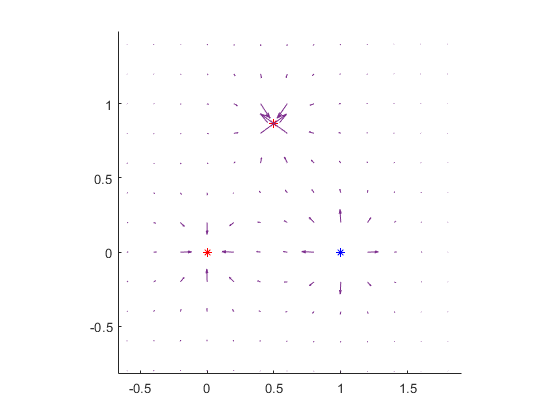
\includegraphics[width=0.5\textwidth]{images/001A.png}
    \caption{Campo eléctrico 3 cargas}
\end{figure}

\begin{lstlisting} [frame=single]
clear; clf; hold off;
xa=-2.1:0.05:2;
ya=-2.1:0.05:2;
k=1.; 
q1 = 1; 
q2 =-1;
q3 =-1;
x1 = 1;     y1 = 0;
x2 = 0;     y2 = 0;
x3 = 0.5;   y3 = sqrt(3) * abs(x2 - x1) / 2;
[x,y]=meshgrid(xa,ya);
z = k*q1./sqrt((x - x1).^2+(y - y1).^2) + ...
    k*q2./sqrt((x - x2).^2+(y - y2).^2) + ...
    k*q3./sqrt((x - x3).^2+(y - y3).^2);
surfl(x,y,z);
zlim([-10,10]); 
\end{lstlisting}

\begin{figure}[H]
\centering
    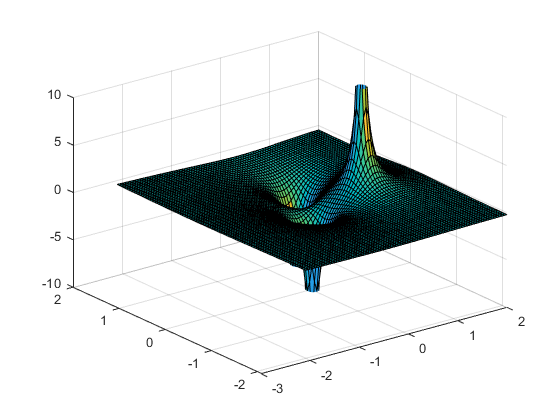
\includegraphics[width=0.5\textwidth]{images/001B.png}
    \caption{Potencial 3 cargas}
\end{figure}

\clearpage
\newpage

\begin{lstlisting} [frame=single]
clear; clf; hold off;
%0.07
%0.0175
xa=-3.1:0.14:3;
ya=-3.1:0.14:3;
k=1.; 
q1 = 1; 
q2 =-1;
q3 =-1;
x1 = 1;     y1 = 0;
x2 = 0;     y2 = 0;
x3 = 0.5;   y3 = sqrt(3) * abs(x2 - x1) / 2;
[x,y]=meshgrid(xa,ya);
z = k*q1./sqrt((x - x1).^2+(y - y1).^2)+...
    k*q2./sqrt((x - x2).^2+(y - y2).^2)+...
    k*q3./sqrt((x - x3).^2+(y - y3).^2);
zmax=max(max(z));
zmin=min(min(z));
dz=(zmax-zmin)/200;
nivel=zmin:dz:zmax;
contour(x,y,z,nivel);
axis equal
\end{lstlisting}

\begin{figure}[H]
\centering
    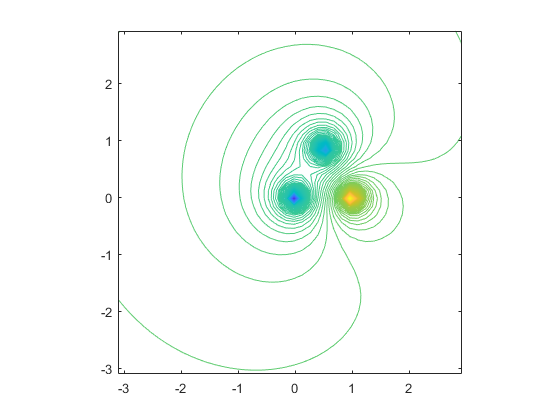
\includegraphics[width=0.9\textwidth]{images/001C.png}
    \caption{Lineas equipotenciales 3 cargas}
\end{figure}

\clearpage
\newpage

\section{Ejercicio 2}

\begin{lstlisting} [frame=single]
clear; clf; hold off;
xa=-3:0.2:3;
ya=-3:0.2:3;
k=1.; 
a = sqrt(3) * 1 / 2;
q  = [2, -1,   -2,    1,   -3,    1];
px = [0, -2, -0.5, -0.5, -1.5, -1.5];
py = [0,  0,    a,   -a,    a,   -a];
[x,y]=meshgrid(xa,ya);
Ex =    k*q(1)*(x - px(1))./((x - px(1)).^2+(y - py(1)).^2).^(1.5)+ ...
        k*q(2)*(x - px(2))./((x - px(2)).^2+(y - py(2)).^2).^(1.5)+ ...
        k*q(3)*(x - px(3))./((x - px(3)).^2+(y - py(3)).^2).^(1.5)+ ...
        k*q(4)*(x - px(4))./((x - px(4)).^2+(y - py(4)).^2).^(1.5)+ ...
        k*q(5)*(x - px(5))./((x - px(5)).^2+(y - py(5)).^2).^(1.5)+ ...
        k*q(6)*(x - px(6))./((x - px(6)).^2+(y - py(6)).^2).^(1.5);
Ey =    k*q(1)*(y - py(1))./((x - px(1)).^2+(y - py(1)).^2).^(1.5)+ ...
        k*q(2)*(y - py(2))./((x - px(2)).^2+(y - py(2)).^2).^(1.5)+ ...
        k*q(3)*(y - py(3))./((x - px(3)).^2+(y - py(3)).^2).^(1.5)+ ...
        k*q(4)*(y - py(4))./((x - px(4)).^2+(y - py(4)).^2).^(1.5)+ ...
        k*q(5)*(y - py(5))./((x - px(5)).^2+(y - py(5)).^2).^(1.5)+ ...
        k*q(6)*(y - py(6))./((x - px(6)).^2+(y - py(6)).^2).^(1.5);
hold on
plot(px(1),py(1),'b*')
plot(px(2),py(2),'r*')
plot(px(3),py(3),'r*')
plot(px(4),py(4),'b*')
plot(px(5),py(5),'r*')
plot(px(6),py(6),'b*')
quiver(x,y,Ex,Ey); axis square
\end{lstlisting}

\begin{figure}[H]
\centering
    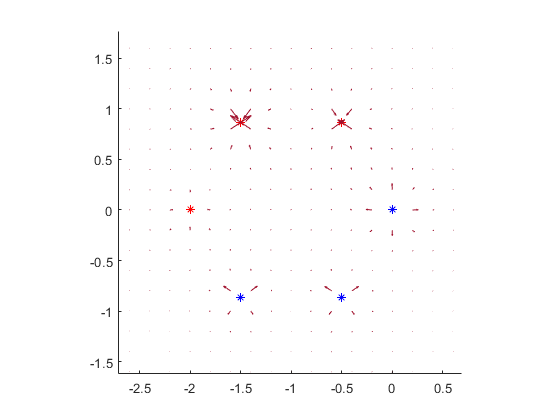
\includegraphics[width=0.5\textwidth]{images/002A.png}
    \caption{Campo eléctrico 6 cargas}
\end{figure}

\clearpage
\newpage

\begin{lstlisting} [frame=single]
clear; clf; hold off;
% 0.048
xa=-2.5:0.048:0.5;
ya=-1.5:0.048:1.5;
k=1.; 
a = sqrt(3) * 1 / 2;
q  = [2, -1,   -2,    1,   -3,    1];
px = [0, -2, -0.5, -0.5, -1.5, -1.5];
py = [0,  0,    a,   -a,    a,   -a];
[x,y]=meshgrid(xa,ya);
z = k*q(1)./sqrt((x - px(1)).^2+(y - py(1)).^2) + ...
    k*q(2)./sqrt((x - px(2)).^2+(y - py(2)).^2) + ...
    k*q(3)./sqrt((x - px(3)).^2+(y - py(3)).^2) + ...
    k*q(4)./sqrt((x - px(4)).^2+(y - py(4)).^2) + ...
    k*q(5)./sqrt((x - px(5)).^2+(y - py(5)).^2) + ...
    k*q(6)./sqrt((x - px(6)).^2+(y - py(6)).^2) ;
surfl(x,y,z);
zlim([-20,20]); 
\end{lstlisting}

\begin{figure}[H]
\centering
    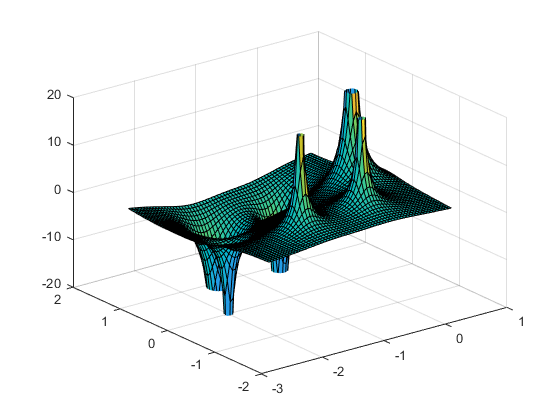
\includegraphics[width=0.5\textwidth]{images/002B.png}
    \caption{Potencial 6 cargas}
\end{figure}

\begin{lstlisting} [frame=single]
clear; clf; hold off;
xa=-5.2:0.0075:3;
ya=-5.2:0.0075:5;
k=1.; 
a = sqrt(3) * 1 / 2;
q  = [2, -1,   -2,    1,   -3,    1];
px = [0, -2, -0.5, -0.5, -1.5, -1.5];
py = [0,  0,    a,   -a,    a,   -a];
[x,y]=meshgrid(xa,ya);
z = k*q(1)./sqrt((x - px(1)).^2+(y - py(1)).^2) + ...
    k*q(2)./sqrt((x - px(2)).^2+(y - py(2)).^2) + ...
    k*q(3)./sqrt((x - px(3)).^2+(y - py(3)).^2) + ...
    k*q(4)./sqrt((x - px(4)).^2+(y - py(4)).^2) + ...
    k*q(5)./sqrt((x - px(5)).^2+(y - py(5)).^2) + ...
    k*q(6)./sqrt((x - px(6)).^2+(y - py(6)).^2);
zmax=max(max(z));
zmin=min(min(z));
dz=(zmax-zmin)/250;
nivel=zmin:dz:zmax;
contour(x,y,z,nivel);
axis equal
\end{lstlisting}

\begin{figure}[H]
\centering
    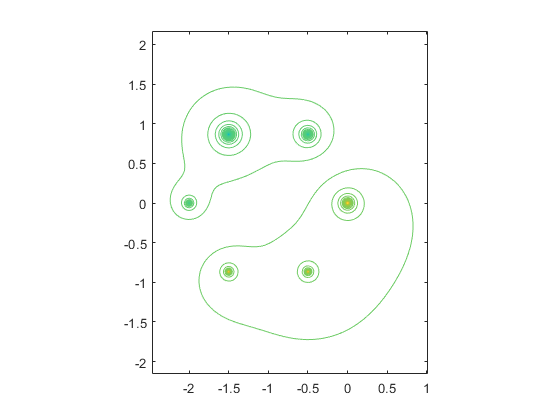
\includegraphics[width=1\textwidth]{images/002C.png}
    \caption{Lineas equipotenciales 6 cargas}
\end{figure}

%%%%%%%%%%%%%%%%%%%%%%%%%%%%%%%%%%%%%%%%%%%%%%%%%%
\clearpage
\newpage

  
\section{Creación del GIF - Potencial 6 cargas}

El gif se encuentra en \textcolor{blue}{  \href{https://drive.google.com/file/d/1sRfifJXut2_qK32Unls1aUzsKwR2ppvl/view?usp=sharing}{Gif}}.
  
  
\begin{lstlisting} [frame=single]
clear; clf; hold off;
% 0.048
h = [1 0.875 0.75 0.625 0.5 0.375 0.25 0.1 0.048 0.024];

drawnow;
frame = getframe(1);
im = frame2im(frame);        
[imind,cm] = rgb2ind(im,256);       
outfile = 'GIF_Potencial_6_Cuerpos.gif';
imwrite(imind,cm,outfile,'gif','DelayTime',0,'loopcount',inf);

for i=1:1:length(h)
    xa=-2.5:h(i):0.5;
    ya=-1.5:h(i):1.5;
    k=1.; 
    a = sqrt(3) * 1 / 2;
    q  = [2, -1,   -2,    1,   -3,    1];
    px = [0, -2, -0.5, -0.5, -1.5, -1.5];
    py = [0,  0,    a,   -a,    a,   -a];
    [x,y]=meshgrid(xa,ya);
    z = k*q(1)./sqrt((x - px(1)).^2+(y - py(1)).^2) + ...
        k*q(2)./sqrt((x - px(2)).^2+(y - py(2)).^2) + ...
        k*q(3)./sqrt((x - px(3)).^2+(y - py(3)).^2) + ...
        k*q(4)./sqrt((x - px(4)).^2+(y - py(4)).^2) + ...
        k*q(5)./sqrt((x - px(5)).^2+(y - py(5)).^2) + ...
        k*q(6)./sqrt((x - px(6)).^2+(y - py(6)).^2) ;
    surfl(x,y,z);
    zlim([-20,20]); 
    title("Potencial 6 cuerpos - h = " + h(i));
    pause(1);
    drawnow;
    frame = getframe(1);
    im = frame2im(frame);        
    [imind,cm] = rgb2ind(im,256);       
    imwrite(imind,cm,outfile,'gif','DelayTime',1,'writemode','append');
end
\end{lstlisting}

\end{document}